\apendice{Documentación de usuario}

\section{Introducción}
Este apéndice sirve como manual de usuario para la aplicación web de demostración desarrollada en el proyecto. El objetivo de este documento es guiar a cualquier persona, independientemente de su nivel técnico, a través del proceso de instalación y uso de la herramienta. Se explicará paso a paso cómo analizar una aplicación Android, cómo interpretar los resultados obtenidos y qué significa cada una de las visualizaciones que ofrece la interfaz, para que la experiencia sea lo más intuitiva posible.

\section{Requisitos de usuario}

La aplicación ha sido empaquetada para que su ejecución sea lo más sencilla posible. Para poder utilizarla en un ordenador local, únicamente es necesario tener instaladas las siguientes herramientas de software:

\begin{itemize}
	\item \textbf{Git:} Un sistema de control de versiones que se usará para descargar el código de la aplicación.
	
	\item \textbf{Git LFS (Large File Storage):} Una extensión de Git necesaria para descargar los archivos de los modelos de IA, que por su gran tamaño no se pueden gestionar de forma convencional.
	
	\item \textbf{Docker:} Una plataforma que permite ejecutar aplicaciones en entornos aislados llamados contenedores. Es la herramienta que nos permitirá lanzar la aplicación con un solo comando, sin preocuparnos por instalar Python ni ninguna de sus dependencias.
\end{itemize}

\section{Instalación}

El método recomendado para ejecutar la aplicación es a través de Docker y utilizando el <<repositorio de despliegue>>\footnote{Enlace al repositorio: \url{https://github.com/dtx1007/streamlit_malware_detection_app}}, que está específicamente preparado para ello. Para obtener información sobre cómo configurar un entorno de desarrollo local, consulte el Apéndice \ref{apendice:documentacion_tecnica}.

Los pasos para el despliegue son los siguientes:

\begin{enumerate}
	\item \textbf{Clonar el repositorio:} Abre una terminal o línea de comandos y ejecuta los siguientes comandos para descargar la aplicación y sus modelos.
	\begin{verbatim}
		# Clona el repositorio de despliegue
		git clone https://github.com/dtx1007/streamlit_malware_detection_app
		cd streamlit_malware_detection_app
		
		# Descarga los archivos grandes (modelos) con Git LFS
		git lfs pull
	\end{verbatim}
	
	\item \textbf{Construir la imagen de Docker:} Una vez dentro del directorio, ejecuta el siguiente comando para que Docker construya la aplicación. Este paso puede tardar unos minutos la primera vez. Se recomienda usar la versión de CPU debido a su mayor compatibilidad.
	\begin{verbatim}
		# Construye la imagen para CPU
		docker build -t streamlit-malware-app:cpu .
	\end{verbatim}
	
	\item \textbf{Ejecutar la aplicación:} Finalmente, lanza la aplicación con el siguiente comando.
	\begin{verbatim}
		# Ejecuta el contenedor de la aplicación
		docker run --rm -p 8501:8501 streamlit-malware-app:cpu
	\end{verbatim}
\end{enumerate}

Tras ejecutar el último comando, la aplicación estará en marcha. Puedes acceder a ella abriendo un navegador web y visitando la dirección: \url{http://localhost:8501}.

\section{Manual del usuario}

Una vez que la aplicación está en ejecución, el usuario se encontrará con una interfaz interactiva diseñada para guiarlo a través del proceso de análisis.

\subsection{Página principal y análisis de una aplicación}

Al entrar a la aplicación se nos muestra la página principal (Figura \ref{fig:streamlit_app_intro}). En la barra lateral izquierda se encuentra el <<panel de control>>, desde donde se pueden subir aplicaciones para ser analizadas y se puede ver el historial de los análisis realizados durante la sesión, junto con un botón para limpiarlo. Para iniciar un análisis, simplemente hay que arrastrar y soltar un archivo o seleccionarlo con el botón <<Browse files>> y, una vez cargado, presionar <<Analyze Uploaded APK>>.

\begin{figure}[h!]
	\centering
	\begin{minipage}[t]{0.45\textwidth}
		\centering
		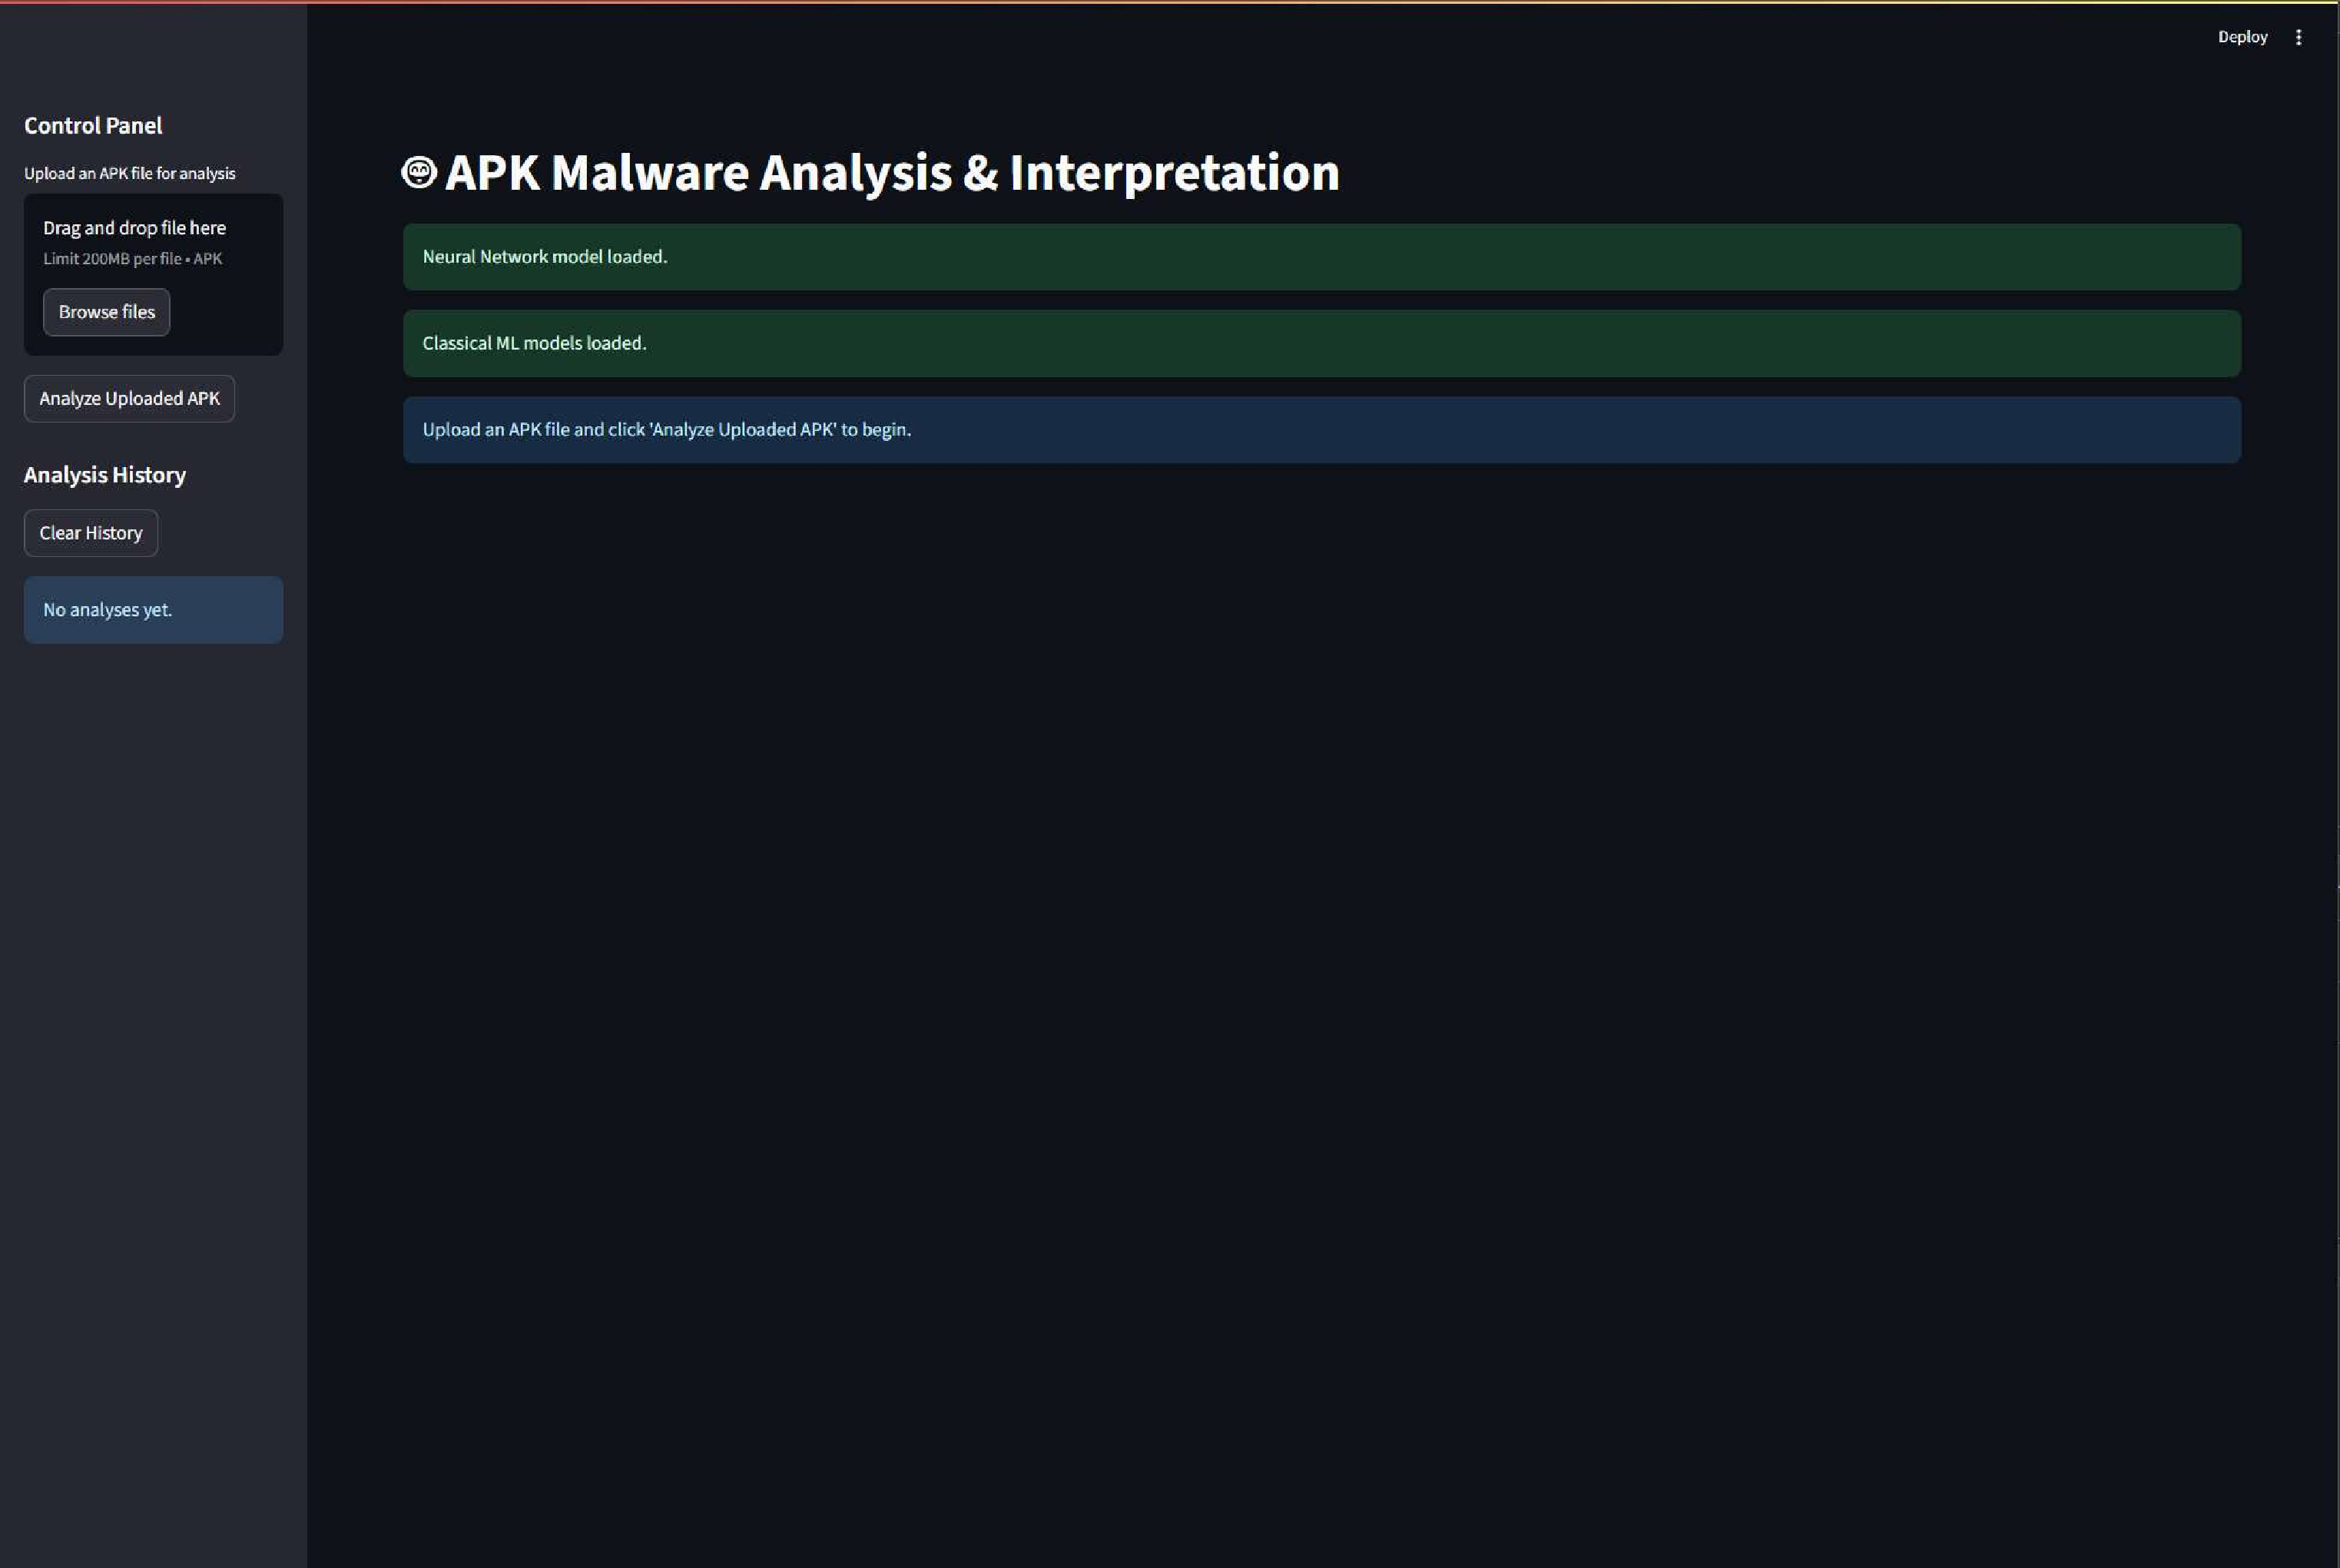
\includegraphics[width=\textwidth]{streamlit_app_intro}
		\caption{Página principal de la aplicación antes de un análisis.}
	\end{minipage}\hfill
	\begin{minipage}[t]{0.45\textwidth}
		\centering
		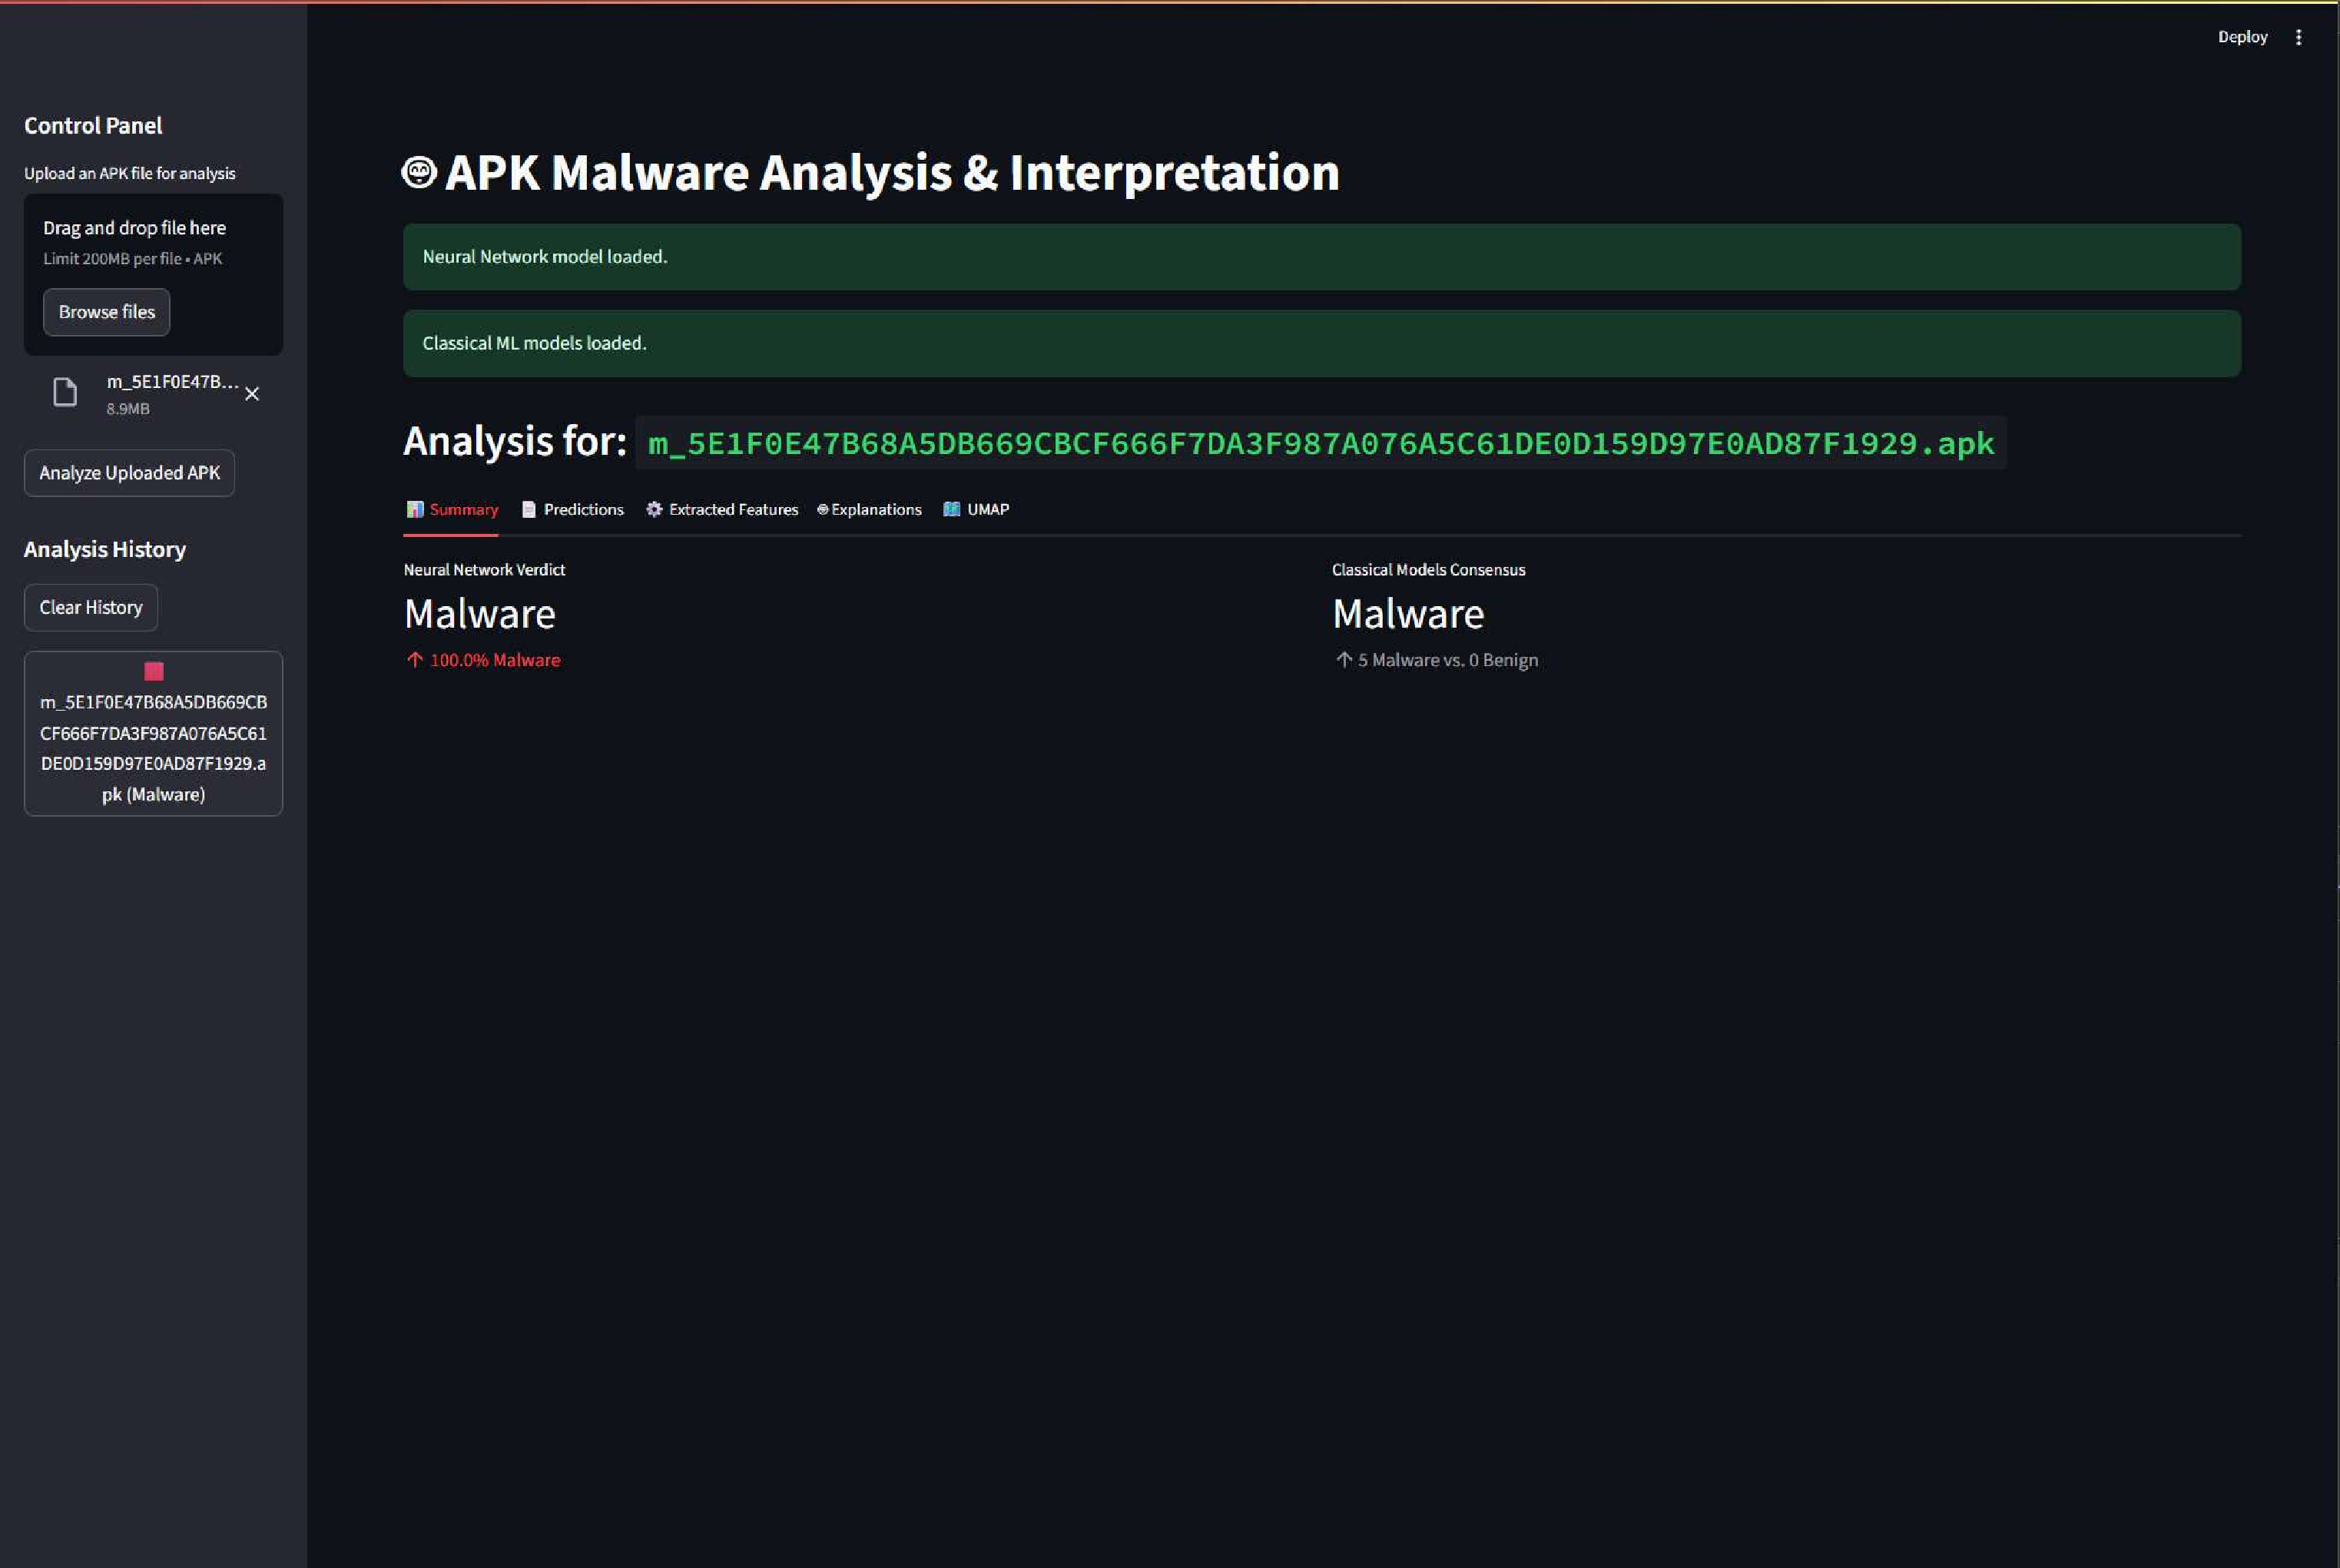
\includegraphics[width=\textwidth]{streamlit_app_main}
		\caption{Página de resumen tras realizar un análisis.}
	\end{minipage}
\end{figure}

Tras unos segundos, la interfaz se actualizará para mostrar los resultados, organizados en varias pestañas. La pestaña inicial, <<Summary>> (Figura \ref{fig:streamlit_app_main}), ofrece un resumen del veredicto final, indicando si el consenso de los modelos apunta a que la aplicación es maliciosa o benigna.

\newpage
\subsection{Pestaña de predicciones}

En esta pestaña (Figura \ref{fig:streamlit_app_prediction}), se ofrece un desglose detallado de la predicción de cada uno de los modelos entrenados. Para cada modelo, se muestra la clase predicha (<<\textit{Malware}>> o <<\textit{Benign}>>) y el nivel de confianza que el modelo tiene en esa predicción, expresado como un porcentaje. Esto permite comparar el veredicto de los diferentes modelos.

\imagen{streamlit_app_prediction}{Pestaña de Predicciones con el detalle de cada modelo.}{1}

\subsection{Pestaña de las características extraídas}

Esta sección ofrece total transparencia sobre la información que el sistema ha extraído de la APK para su análisis, permitiendo entender en qué datos se basan las predicciones. Se divide en varias subpestañas.

La primera, <<AndroidManifest>> (Figura \ref{fig:streamlit_app_extraction_1}), muestra los componentes clave declarados en el manifiesto de la aplicación: los permisos que solicita (acceso a contactos, internet, etc.), las actividades (las diferentes <<pantallas>> que hay en la aplicación), los servicios (procesos en segundo plano) y los receptores (componentes que responden a eventos del sistema).

\imagen{streamlit_app_extraction_1}{Pestaña de características: Sección del AndroidManifest.}{0.85}

La subpestaña <<Code Analysis>> (Figura \ref{fig:streamlit_app_extraction_2}) detalla las llamadas a la API, que son las funciones externas a la aplicación que esta usa, y el recuentos de los distintos \textit{opcodes}, que son las instrucciones de bajo nivel que el sistema es capaz de ejecutar.

\imagen{streamlit_app_extraction_2}{Pestaña de características: Sección de análisis de código.}{0.85}

Finalmente, <<File Properties>> (Figura \ref{fig:streamlit_app_extraction_3}) muestra algunas propiedades del archivo como su tamaño y su \textit{fuzzy hash}. La sección <<Advanced>> revela cómo toda esta información se convierte en los números que el modelo realmente utiliza, incluyendo la representación final del \textit{embedding}.

\imagen{streamlit_app_extraction_3}{Pestaña de características: Propiedades del archivo y datos procesados.}{1}

\newpage
\subsection{Pestaña de explicaciones (interpretabilidad)}
Esta es una de las pestañas más importantes, ya que intenta responder a la pregunta: <<¿Por qué el modelo ha tomado esta decisión?>>. Utiliza la técnica SHAP para visualizar el razonamiento del modelo. Primero, se debe seleccionar en el menú desplegable el modelo que se desea analizar.

\imagen{streamlit_app_shap_1}{Pestaña de explicaciones: Gráficos de interpretabilidad global del modelo.}{1}

La sección muestra primero el análisis local (Figura \ref{fig:streamlit_app_shap_1}), que se centra exclusivamente en la APK que se acaba de analizar. Hay dos gráficos en esta sección, el primero, llamado gráfico de <<fuerzas>> muestra el <<tira y afloja>> de las características: las que están en rojo han empujado la predicción hacia \textit{malware}, mientras que las que están en azul han empujado hacia benigno. Por otro lado, el segundo de los gráficos, que se encuentra dejado del de <<fuerzas>> se llama gráfico en <<cascada>> y muestra exactamente la misma información pero de manera desglosada para que sea más sencillo entender qué ha influenciado más al modelo en realizar la predicción actual. Los valores de ambas gráficas se expresan en tanto por uno pero representan la <<porción>> de probabilidad de la predicción que han ayudado a conseguir.

\imagen{streamlit_app_shap_2}{Pestaña de explicaciones: Gráfico de interpretabilidad local para la APK analizado.}{1}

A continuación, se muestra el análisis global (Figura \ref{fig:streamlit_app_shap_2}). Hay 3 gráficos en esta sección. El primero de ellos es un gráfico de barras, el cual representa la <<importancia>> absoluta (es indepediente de la predicción) de las diferentes características de entrada del modelo y muestra de forma visual cuales son más importantes para este en términos general. El siguiente gráfico recibe el nombre de <<enjambre>> y muestra una vista más detallada del comportamiento del modelo: cada punto es una predicción y muestra cómo el valor de cada  característica empuja la decisión hacia <<\textit{malware}>> (valores SHAP positivos, hacia la derecha) o <<benigno>> (negativos, a la izquierda). Finalmente, está el <<mapa de calor>> el cual muestra cuales han sido las características más importantes para el modelo a la hora de realizar diferentes predicciones.

\imagen{streamlit_app_shap_3}{Pestaña de explicaciones: Gráficos de dependencia de SHAP.}{1}

Por último, la Figura \ref{fig:streamlit_app_shap_3} muestra un gráfico interactivo conocido como gráfico de <<fuerzas>> global, el cual se forma apilando todos los gráficos de <<fuerzas>> de todas las explicaciones de referencia. A su vez, se muestran los gráficos de <<dependencia>> de las características con mayor importancia para el modelo, contrastadas con la característica de mayor importancia, estos gráficos muestran el valor que tenía la característica dada respecto del valor de la predicción (valor SHAP), de tal manera se puede saber si para un valor dado de dicha característica la predicción suele ser <<\textit{malware}>> o <<benigna>>. A su vez, el color indica el valor que tenía la característica de contraste en esa predicción, esto ayuda a encontrar posibles interacciones entre las diferentes características.

\subsection{Pestaña de UMAP}

Esta última pestaña (Figura \ref{fig:streamlit_app_umap}) ofrece una visualización acerca del espacio de \textit{embeddings} del modelo. Es decir, representa de forma visual dónde cae la predicción dentro de su espacio de \textit{embeddings}.

\imagen{streamlit_app_umap}{Pestaña UMAP: Proyección 2D del espacio de \textit{embeddings}.}{1}

Este gráfico muestra dónde se posiciona una aplicación dada dentro del espacio de <<embeddings>> del modelo, dicho de otra forma, a grandes rasgos, el modelo aprende a <<agrupar>> las aplicaciones maliciosas y separarlas de las aplicaciones benignas, este gráficos muestra precisamente donde a colocado en este caso el modelo a la muestra actual.
